\documentclass{article}
\usepackage{url}
\usepackage{amssymb,amsfonts,amsmath,amsthm,mathtools}
\usepackage{adjustbox}
\usepackage{float}
\usepackage{caption}
\usepackage{mdframed}
\usepackage{lmodern}
\usepackage{bm,bbold}
\usepackage{xfrac, nicefrac}
\usepackage{lmodern}
\usepackage{enumitem}
\usepackage[margin=60pt]{geometry}
\pdfinclusioncopyfonts=1
\captionsetup{width=0.85\textwidth}
\usepackage{pgfplots, pgf,tikz}
\usepgfplotslibrary{fillbetween}
\pdfinclusioncopyfonts=1
\captionsetup{width=0.85\textwidth}

\usepackage{xcolor}
\definecolor{RED}{HTML}{EB6231}
\definecolor{YELLOW}{HTML}{E29D26}
\definecolor{BLUE}{HTML}{5D80B4}
\definecolor{LIGHTGREEN}{HTML}{6ABD9B}
\definecolor{GREEN}{HTML}{8FB03E}
\definecolor{PURPLE}{HTML}{BE1E2D}
\definecolor{BROWN}{HTML}{A97C50}
\definecolor{PINK}{HTML}{DA1C5C}

\newcommand{\specialcell}[2][c]{%
	\begin{tabular}[#1]{@{}c@{}}#2\end{tabular}}

\DeclareMathOperator{\E}{\mathbb{E}}
\newcommand{\der}{\mathrm{d}}
\newcommand{\e}{\mathrm{e}}
\newcommand{\angstrom}{\text{\normalfont\AA}}

% Time, effective population size and mutation rate.
\newcommand{\Ne}{N_{\mathrm{e}}}
\newcommand{\dnds}{\omega}
\newcommand{\Nsite}{\text{n}}
\newcommand{\Nsites}{\text{n}}
\newcommand{\site}{\text{i}}
\newcommand{\Nstate}{\text{K}}

\newcommand{\x}{x}
\newcommand{\eq}{^{*}}
\newcommand{\dx}{\delta \x}
\newcommand{\s}{s}
\newcommand{\deltaG}{\Delta G}
\newcommand{\deltaGMin}{\alpha}
\newcommand{\deltadeltaG}{\Delta \deltaG}

\newcommand{\ci}{\mathbb{S}_{t}}
\newcommand{\cj}{\mathbb{S}_{t}'}
\newcommand{\itoj}{\ci, \cj}
\newcommand{\setNeighbors}{\mathcal{M}\left(\ci\right)}
\newcommand{\setNonSynNeighbors}{\mathcal{N}\left(\ci\right)}
\newcommand{\setSynNeighbors}{\mathcal{S}\left(\ci\right)}
\newcommand{\submatrix}{q}

\begin{document}
\title{Substitution rate responses to changes in effective population size.}
\author{T. Latrille, N. Lartillot}
\maketitle
 
\abstract{
The quasi-neutral theory of evolution asserts that the effective population size ($\Ne$) plays an important role in shaping the evolution of molecular sequences.
One consequence is that $\Ne$ modulates selection, such populations with high $\Ne$ would have stronger purifying selection, due to the decrease of random drift.
In molecular sequence, this effect translates in the decrease in the substitution rate of selected mutations relative to the substitution rate of neutral mutation ($\dnds$) with respect to $\Ne$.
Such theoretical prediction had been observed in empirical data across many clades.
However, several studies failed to observe such response of $\dnds$ to changes in $\Ne$, or with weak strength or direction.
Computational models of protein folding have observed that $\dnds$ can be independent of $\Ne$, which can mathematically be proven under certain assumptions.
Moreover, non-equilibrium properties can imply that an increase of $\Ne$ can result first in an increase of $\dnds$ and then a decrease.
Together, assumptions about the mapping of sequence to fitness can display a variety of behaviors in the $\dnds$ responses to changes in $\Ne$.
Our goal in this present work is to provide theoretical tools to derive the relationship between $\Ne$ and $\dnds$ in the context of a genotype-phenotype-fitness map.
We apply our framework in the special case of fitness proportional to the probability of protein folding.
Our compact theoretical results are supported by more complex simulations using 3d structure of proteins.
We assert that models based on the probability of folding are at odds with empirically results obtained on the $\Ne$-$\dnds$ relationship in population genetic dataset.
However, our framework applied to the case of non-specific interactions between proteins suits more the empirical data.
We also stress the importance of epistatic interactions in the $\Ne$-$\dnds$ relationship, such that it determines to time to reach a new equilibrium, and that models without epistasis might be too slow to be realistic.
}
\section*{Introduction}
Molecular sequences differ across species due to the particular history of DNA substitutions along each specie's respective lineage.
These substitutions in molecular sequences are the result of the interplay between evolutionary forces such as mutation, selection and random genetic drift.
These forces have effects at different levels, mutations are carried by molecular sequence, selection is beared by individual's fitness, and random genetic drift is a population effect.
The strength of random genetic genetic, or stochastic sampling of mutations, is less pronounced in lineage with high effective population size ($\Ne$), and as a consequence the purification by selection of deleterious mutations is more effective.
Such idea has emerged in the framework of quasi-neutral theory of evolution, whereby predicting a decrease in the substitution rate per unit of time of selected mutations along a lineage with higher $\Ne$ \cite{Ohta1972, Ohta1992}.
This prediction is valid under the assumption that most mutations are deleterious and that their selective effect on individuals are drawn from a fixed distribution \cite{Welch2008}.
Furthermore, this prediction assumes a constant mutation rate per unit of time, but such assumption can be relaxed by normalizing the substitution rate of selected mutations by the substitution rate of neutral mutations such as to discard this confounding factor \cite{Ohta1972}.
This relative substitution rate of selected mutations, called $\dnds$ is this study, is a theoretical macroscopic observable in molecular sequence evolution, given we can separate selected and neutral mutations.
Practically, $\dnds$ can be approximated in protein-coding DNA sequences, where selected mutations are the non-synonymous changes affecting the amino-acid sequence, and the non-synonymous mutations are supposedly neutral, this statistic is called $dNdS$.\\
% \dnds decrease with \Ne under the assumption of fixed DFE

The context of protein coding sequence fostered another modeling of selection, based on genotype-fitness map instead of distribution of fitness effects.
In such approach, the selective effect of a mutation depends on the fitnesses of both source and target amino-acids involved on the mutation \cite{Halpern1998}.
For example, if the target amino-acid has an higher fitness, the selective effect of the mutation is positive, and reciprocally negative for lower fitness.
Such modeling approach account for higher substitutions rate between amino-acid with similar bio-chemical properties.
Fundamentally, in such framework the fitness depends solely on the actual genotype, not on the trajectory of mutations leading to this sequence.
Even thought the modeling approach is substantially different, assuming each site of the sequence has its own genotype-fitness map also predicts a negative correlation between $\dnds$ and $\Ne$ \cite{Spielman2015a, DosReis2015}.\\
% \dnds decrease with \Ne under the assumption site fitness landscape

Empirically, fluctuation of $\dnds$ along lineages of phylogenies have been inferred using protein-coding DNA alignments \cite{Yang2001, Zhang2004}.
Subsequently, inference methods combining molecular sequences and lineage specific quantitative traits have asserted that $\dnds$ correlates positively with longevity and body mass, traits which have been sampled only in the extant lineages \cite{Lartillot2011,Weber2014}.
Moreover, longevity and body mass are proxies of $\Ne$, with low $\Ne$ corresponding to lineage with a large body size and extended longevity \cite{Romiguier2014}.
As such, empirical evidences suggest a negative correlation between $\dnds$ and $\Ne$, confirming the theoretical prediction of the quasi-neutral theory of evolution.
However, this correlation could not be replicated across all experiments, and depending on the clade or the potential biases taken into account, the correlation could be in the inverse direction or not statistically significant \cite{Figuet2016}.\\
% \dnds decrease with \Ne empirically, but not always

Mitigated empirical evidence that $\dnds$ decrease with $\Ne$ encouraged alternative explanatory mechanism \cite{Lanfear2014}.
One striking result proved that $\dnds$ can independent of $\Ne$, when fitness is a function of a phenotype and that such phenotype is equimutable.
Equimutability states that the probabilities of phenotype changes due to mutations is independent the current phenotype of the individual \cite{Cherry1998}.
Such argument has been invoked in the \textit{in silico} observation that $\dnds$ is seamingly independent of $\Ne$ if the protein thermodynamic stability is computed using a 3D structural model of the protein, and that the fitness is proportional to the folding probability of the protein \cite{Goldstein2013}.
The given explanation is that probabilities of changes in free energy of folding ($\deltadeltaG$) is independent of the current free energy ($\deltaG$), which is considered an equimutable phenotype.\\
% Explanation could be that \dnds is independent of \Ne

However, this assumption is relatively strong, as for example if a protein is completely stable, only destabilizing mutations can occur, and more generally the probabilities of destabilizing mutational events is dependent on the actual composition of the protein.
Under the assumption that fitness relates to protein stability, and that such stability if a function of the genotype, the theoretical $\dnds$ relationship to $\Ne$ is unknown.
The goal of this study is to derive the $\dnds$ relationship to $\Ne$ to intrinsic molecular parameters of the model.
More generally, we develop mathematical tools to derive the $\dnds$ relationship to $\Ne$ in the context of a genotype-phenotype-fitness map.
With such results, we stress to test the assumption that protein stability is a proxy of fitness in the light of empirical data.\\
% The assumptions are strong, we want to relax equimutability which is unlikely

Orthogonally to the relationship between $\dnds$ and $\Ne$, independent studies have argued that protein abundance is also a predictor of $\dnds$.
As such, we also seek to derive the $\dnds$ relationship to protein abundance, and discuss the empirical implication.\\
% \dnds is relationship to protein abundance

Lastly, the theoretical results discussed so far are all obtained when the balance between mutation, selection and drift is at equilibrium.
However, under a model of site-dependent genotype-fitness map, an increase in $\Ne$ leads first to an increase of $\dnds$ due to adaptive selection, and subsequently a decrease in $\dnds$ due to stronger purifying selection \cite{Jones2016}.
Studying only equilibrium properties can thus be misleading, and the dynamical response of $\dnds$ to changes in $\Ne$ must also be addressed by our model.\\
% Result at equilibrium, what about dynamical properties?

\section*{Results}
\subsection*{Theoretical approximations}
In this section we present an analytical approximate solution for the change in $\dnds$ at equilibrium after a change in $\Ne$.
The main results are given in a general case of any phenotype-fitness map, and also derived in the specific case of fitness proportional to the total amount of folded protein.
All development are available in Supplementary Materials in the most general case.
The first step define the relationship from genotype to fitness, through an intermediary phenotype.
The second step present the equation of the phenotype at equilibrium, when evolutionnary forces of mutation, selection and genetic drift compensate each others.
Finally, an approximate response of $\dnds$ to changes in $\Ne$ is derived from the equilibrium equation. \\

We base our work on numerical model of protein stability \cite{Williams2006, Goldstein2011, Pollock2012}, on which we make simplifying assumptions to derive analytical equations.
In the original model, the protein stability is the difference in free energy between folded and unfolded conformations, called $\deltaG$ in kcal/mol.
Technically, the free energy of the folded are unfolded conformations are computed using $3$D conformations of the protein.
In such model, the stabilizing or destabilizing effect of an amino-acid at a particular site depends on the amino-acids present in the vicinity in $3$D conformation.\\

We approximate this model such that the destabilizing effect of an amino-acid does not depend on a $3$D representation of the protein, but each site contribute independently to $\deltaG$.
With such approximation, at a given site of sequence each amino-acid is either stabilizing or destabilizing the protein, and an unstable amino-acid contribute to an excess of $\gamma > 0$ (in kcal/mol) to $\deltaG$ compare to a stable amino-acid.
If all amino-acids of the sequence are stable, $\deltaG$ equal to $ \alpha < 0$. 
In this model, the more compact phenotype summarizing the genotype is the proportion of unstable amino-acid in the sequence, defined as $0 \leq \x \leq 1$, and $\deltaG$ is a linear function of $\x$:
\begin{align}
\deltaG (\x) = \alpha + \Nsite \gamma \x,
\end{align}
where $\Nsite$ is the number of sites in the sequence. \\

From a given genotype, mutations changing the sequence have various effect, they can increase or decrease the proportion of unstable amino-acid, or do nothing if the mutation is between both unstable (or equivalently stable) amino-acids.
To derive the probabilities of such events to occur, we also make the simplyfing assumption that the transition between amino-acids are equiprobable and only one amino-acid is stable and the $19$ others are unstable.
Altogether, any mutation in the sequence can then have a phenotypic effect of $0$ or $\dx=\sfrac{1}{\Nsite}$, and the probabilities of transition are:
\begin{gather}
\begin{cases}
\dx &\text{ with probability } 1-x, \\
0 &\text{ with probability } \frac{18 \x }{19}, \\
-\dx &\text{ with probability } \frac{\x}{19}.\\
\end{cases} \label{eq:proba}
\end{gather}
In the extreme case of optimal phenotype ($\x = 0$), only destabilization mutations are proposed.
Moreover, the probability to propose stabilizing mutation (effect $-\dx$), or between unstable amino-acids (effect $0$) is proportional to $\x$. 
Once obtained the phenotypic effects of mutations and their probabilities, definition of the phenotype-fitness map is necessary derive the selective effect of mutations.\\
 
Subsequent equations are valid for the more general case where the Wrightian fitness is a log-concave differentiable function $f$ of phenotype $\x$.
As an example, we develop the argument when the Wrightian fitness of an individual is the proportion of protein in folded conformation.
This fitness function is motivated in part that a protein must be folded to perform its function, but can also be justified by the toxic effect of misfolded proteins in the cytoplasm. 
This fitness is then given by the Fermi Dirac distribution and is typically close to $1$, leading to a first-order approximation\cite{Goldstein2011}: 
\begin{align}
f(\x) = \dfrac{1}{1 + e^{\beta (\alpha + \Nsite \gamma \x)}},\\
\Rightarrow f(\x) \simeq 1 - e^{\beta (\alpha + \Nsite \gamma \x)}, 
\end{align}
where $\alpha$ and $\gamma$ are defined as above, and the fixed parameter $\beta$ is $1.686$ mol/kcal at room temperature.
Destabilizing mutations are selected against with a negative selection coefficient which can be approximated by:
\begin{align}
s & \simeq \frac{1}{\Nsite}\frac{ \partial \ln f(\x) }{\partial \x} \label{eq:s} \\
\Rightarrow s & \simeq - \beta \gamma e^{\beta (\alpha + \Nsite \gamma \x)} \label{eq:s-unfolded}
\end{align}

With the complete genotype-phenotype-fitness map defined (see Figure \ref{fig:NeChangeInfluence}, left panel), one can study the evolutionary processes unfolds.
Starting from an optimal sequence, destabilizing mutations will reach fixation and accumulate until the selection coefficient against new deleterious mutations is too strong, a point of equilibrium called marginal stability.
Most importantly the probability of fixation of mutations is affected by genetic drift, parameterized by effective population size ($\Ne$).
Altogether, at the equilibrium between mutation, selection and drift, the selection coefficient of new advantageous and deleterious mutations reaching fixations are expected to be null on average.
Formally, and after simplification, the equilibrium phenotype denoted $\x\eq$ is given by the equation:
\begin{align}
\ln \left( \frac{1 - \x\eq}{\x\eq} \right) + \ln (19) & \simeq - \frac{4\Ne}{\Nsite} \frac{ \partial \ln f(\x\eq) }{\partial {\x\eq}}, \\
\Rightarrow \ln \left( \frac{1 - \x\eq}{\x\eq} \right) + \ln (19)  & \simeq 4\Ne \beta \gamma e^{\beta (\alpha + \Nsite \gamma \x\eq)}. \label{eq:equilibrium}
\end{align}
This equation cannot be solved explicitly for $\x\eq$, but an intuition on the consequences of change in $\Ne$ to the equilibirum phenotype $\x\eq$ is given in Figure \ref{fig:NeChangeInfluence} (right panel). \\
\begin{figure*}[htb!]
	\begin{mdframed}
		\centering
		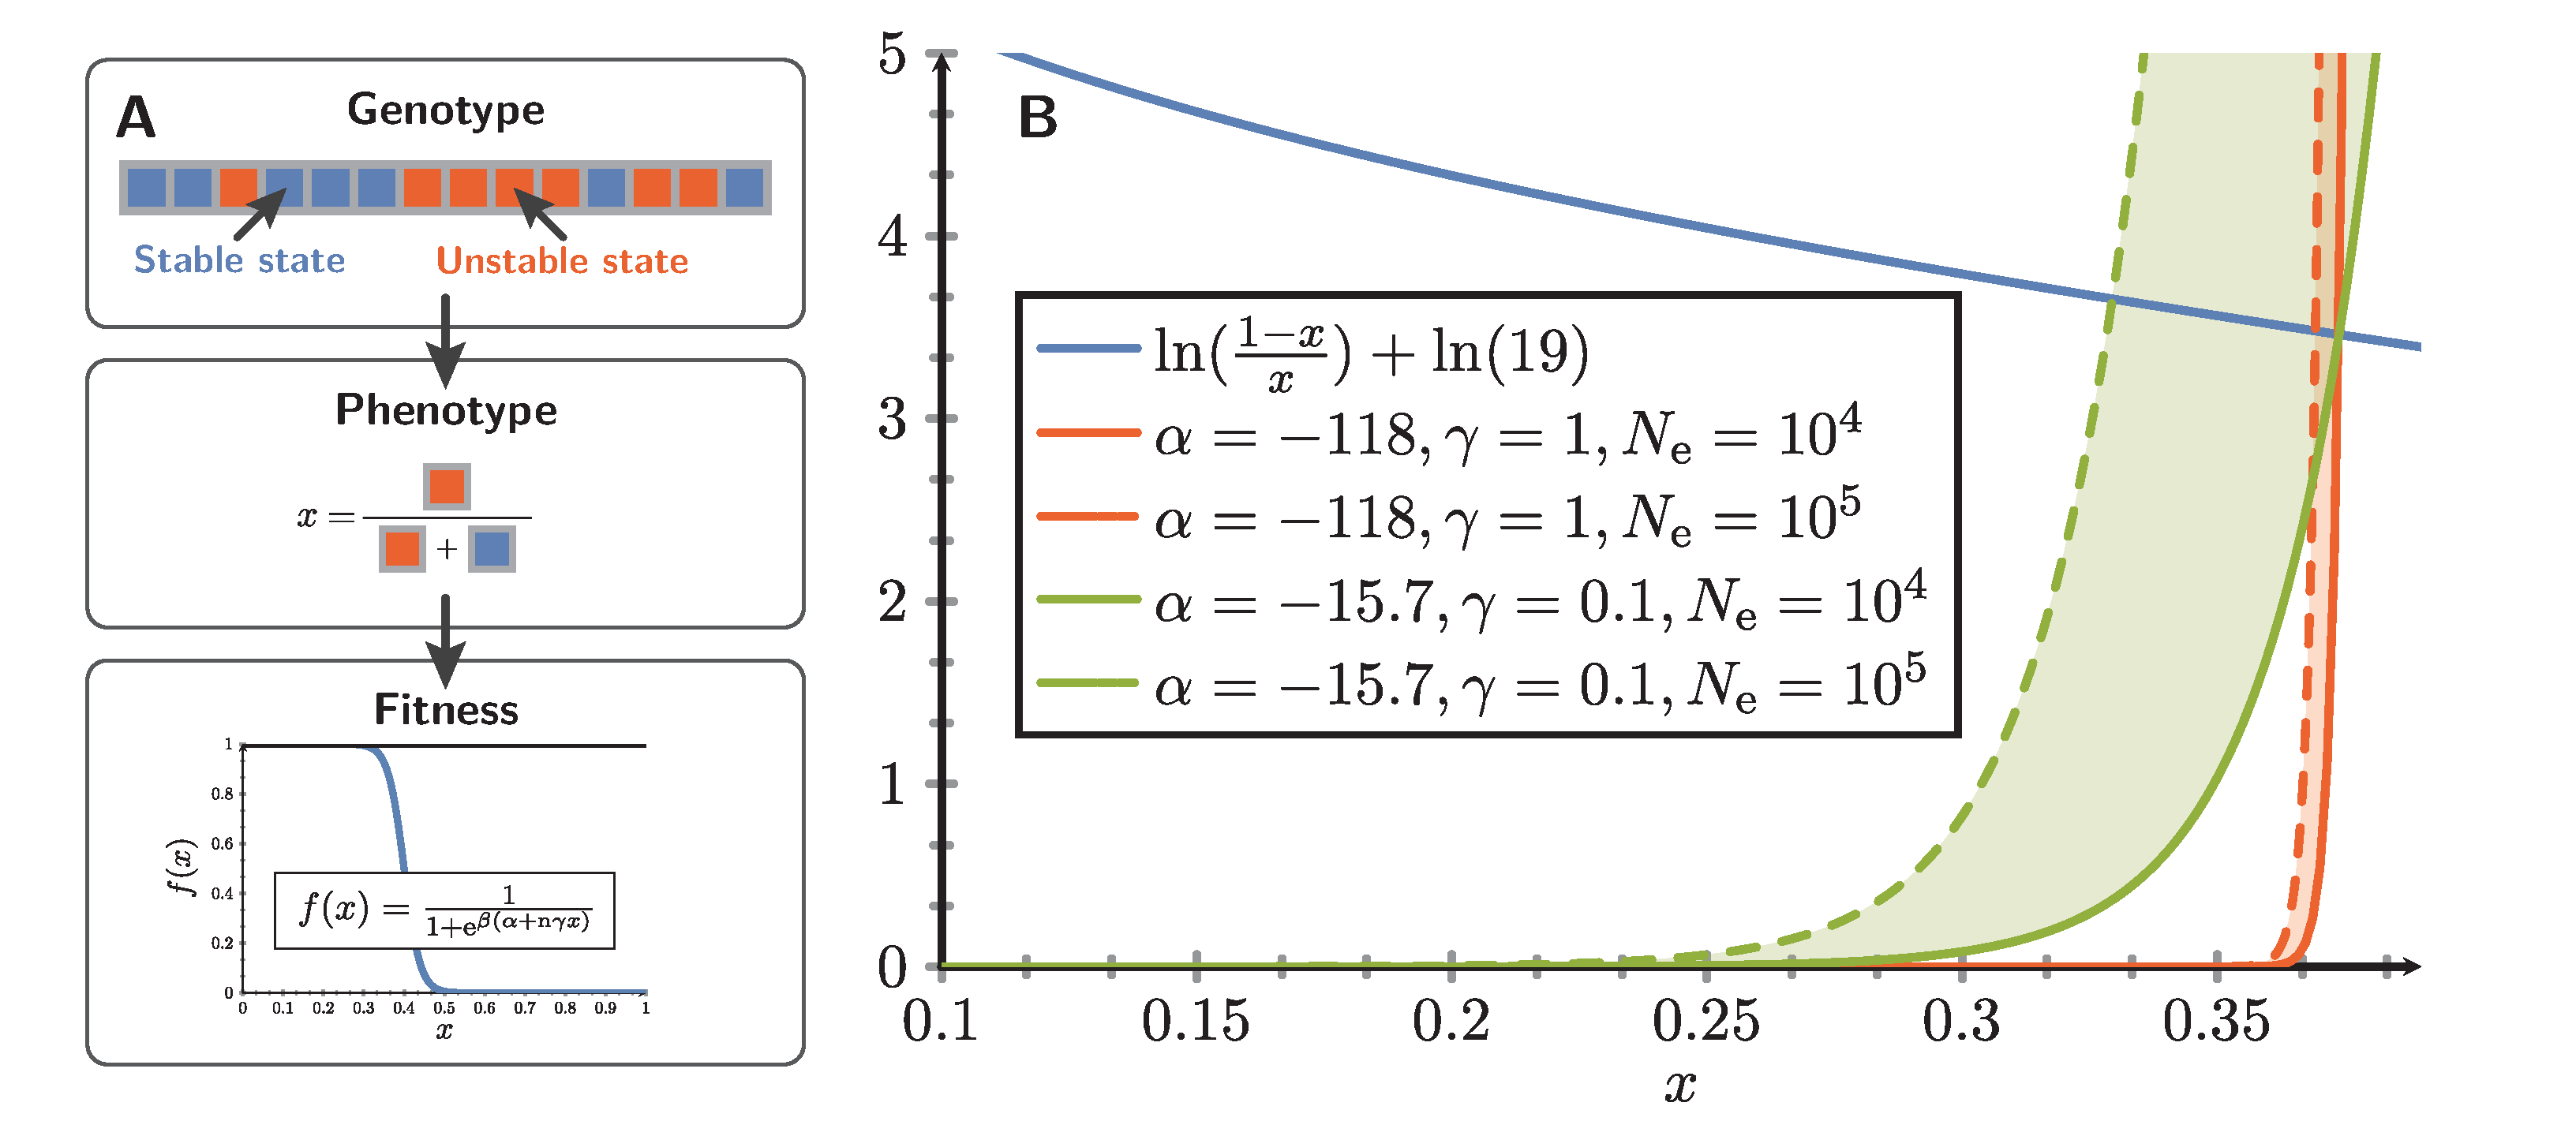
\includegraphics[width=0.9\textwidth, page=1] {artworks/theoretical.pdf}
		\caption{
			\textbf{Theoretical model.}
			Panel A. Illustration of the Genotype-phenotype-fitness map. The phenotype ($\x$) is a real-valued summary of the genotype, and is defined in our model as the fraction of unstable sites in the sequence. The fitness is a decreasing log-concave function of the phenotype.
			Panel B. Illustration of the $\dnds$ elasticity after a change in $\Ne$. The equilibrium $\x\eq$ is determined by the equation $\ln(\frac{1 - \x\eq}{\x\eq}) + \ln(19)=4\Ne \beta \gamma e^{\beta (\alpha + \Nsite \gamma \x\eq)}$. The right-hand side of the equation increases exponentially with $\x$ where $\Nsite \gamma$ is the exponential growth rate. Thus when $\Nsite \gamma$ is large (red solid line), increasing $\Ne$ (red dotted line) only changes subtly $\x\eq$ (x-axis of the crossing with the blue solid line). On the other hand, when $\Nsite \gamma$ is low (green solid line), increasing $\Ne$ (green dotted line) involve a stronger response of $\x\eq$. Moreover, changes in $\x\eq$ reflects the changes in $\dnds$ since both are related by a monotonous function (equation \ref{eq:dnds}). The value of $\alpha$ has been chosen given all other parameters such that the solid lines all cross at the same point.
		}
		\label{fig:NeChangeInfluence}
	\end{mdframed}
\end{figure*}

Moreover, at equilibrium we can derive the expected substitution rate of mutations changing the sequence, and by normalizying by the substitution rate of neutral mutations, $\dnds$ simply approximates to:
\begin{gather}
\dnds \simeq \x\eq \label{eq:dnds}
\end{gather}
This simple approximation is due to substitutions at unstable sites (proportion $\x\eq$) to one of the other unstable amino-acids, which are effectively neutral and compose the largest proportion of proposed mutations with substantial probability of fixation (see equation \ref{eq:proba}).\\

From the equilibrium equation \ref{eq:equilibrium}, differential calculus allow to derive the response of $\x\eq$ and ultimately $\dnds$ after a change in $\Ne$.
We define the elasticity $\chi$ as slope of the $\dnds$ response to changes in $\Ne$ in log scale, which simplify to a compact equation: 
\begin{align}
\chi = \frac{ \der \dnds}{\der \ln (\Ne)} & \simeq - \frac{\frac{ \partial \ln f(\x\eq) }{\partial {\x\eq}}}{\frac{ \partial^2 \ln f(\x\eq) }{\partial {\x\eq}^2}}, \\
\Rightarrow \chi & \simeq -\dfrac{1}{\beta \Nsite \gamma}.
\end{align}
The elasticity is the ratio of first to the second derivative of the log-fitness function, taken at the equilibrium phenotype. To note, this elasticity is strictly negative for decreasing log-concave fitness functions, asserting that $\dnds$ is a decreasing function of $\Ne$.
In the case of fitness equal to the folded proportion, $\chi$ is independent of $\x\eq$, meaning that $\dnds$ is linearly decreasing with $\Ne$ in log space.
Moreover, only the compound parameter $\beta \gamma \Nsite$ has an impact on the slope of the linear relationship, where only $\gamma$ and $\Nsite$ are free parameters. \\

Other parametrization of the fitness function shed light on the robustness of the theoretical results.
If the selective coefficient itself is not equal (equation \ref{eq:s-unfolded}) but proportional to the total amount of misfolded protein, and the expression level of the protein is denoted $y$, then the response of $\dnds$ to changes in $\Ne$ is the same as the response to changes in $y$ (See Supplementary Materials):
\begin{align}
s & \propto - \beta \gamma y  e^{\beta(\alpha + \gamma \Nsite \x)} \\
\Rightarrow \chi = \frac{ \der \dnds}{\der \ln (y)} & \simeq -\dfrac{1}{\beta \Nsite \gamma}.
\end{align}
Meaning we should observe the same relationship between $\dnds$ and $\Ne$ that between $\dnds$ and expression level.\\

Under empirically relevant value of $\Nsite=300$ sites and $\gamma=1.0$ kcal/mol \cite{Zeldovich2007}, the elasticity $\chi \simeq -0.002$.
In other words, for a increase in $\Ne$ of $4$ orders of magnitude, $\dnds$ decrease approximately of $0.01$, a subtle relationship that requires laborious  effort to be detected in simulated data, and large amount of empirical data with few bias and noise to be detectable.

\subsection*{Simulations confirmation}
In order to test the soundness of our compact theoretical results, we relaxed several assumptions by simulating DNA sequences evolution (See Methods), under various range of $\Ne$ and reporting the average $\dnds$ observed along the computation. 
With respect to mutation, we assumed that all amino-acids transition are equiprobable, in other word the complexity of the genetic code is not taken into account.
Simulating evolution of DNA sequence, and taking into account a matrix a mutation rate between nucleotide allow to test directly the robustness of the results to this assumption.
Furthermore, with regards to fitness, we assumed that all unstable amino-acids are equivalently unstable.
This assumption is relaxed by choosing for every site of the sequence one stable amino-acid, and the impact on the phenotype ($\x$) of other amino-acids is not binary, but scaled by the Grantham amino-acid distance \cite{Grantham1974}.
Also, the number of sites in the sequence ($\Nsite$) is assumed to be large such that the selection coefficient is well approximated by the fitness derivative (equation \ref{eq:s}).
The robustness of such approximation is test in the simulations with sequences of a finite number of sites ($\Nsite=300$).\\

Simulations demonstrate that the relation between $\dnds$ and log-$\Ne$ is linear, and that the slope of the linear regression match the expected theoretical value (See Figure \ref{fig:GoldsteinVsToy}, panel B).
Secondly we observe that effect of the parameter $\alpha$ is subtle on the slope of the linear regression, as expected also theoretically (See Figure \ref{fig:GoldsteinVsToy}, panel A).
Decreasing $\alpha$ (to more negative values) increases $\dnds$, by shifting the equilibrium to higher $\x\eq$ since more unstable sites are fixed before reaching the point of marginal stability.\\

Finally, we relaxed our assumption that each site of the sequence contribute independently to $\deltaG$, by taking into account the $3$D structure of protein.
We implemented the original model \cite{Williams2006, Goldstein2011, Pollock2012}, in which the free energy of the folded are unfolded conformations are computed using $3$D structures of the protein conformations and pairwise contact potential energies between neighboring amino-acid residues \cite{Miyazawa1985} (see Supplementary Materials).
The original works claimed that under such $3$D model $\dnds$ is independent of $\Ne$ \cite{Goldstein2013}.
Using extensive simulations, we argue instead that $\dnds$ is approximately linear with log-$\Ne$ (see Figure \ref{fig:GoldsteinVsToy}, panel C).
Moreover, the observed slope match the theoretical value considering $\deltadeltaG = 1.0$ kcal/mol for destabilizing mutations and $\Nsite=300$. 
In such experiment, $\alpha=-118$ kcal/mol as it is the $\deltaG$ of the optimal sequence of $300$ sites \cite{Goldstein2011}.
\begin{figure*}[htb!]
\begin{mdframed}
\centering
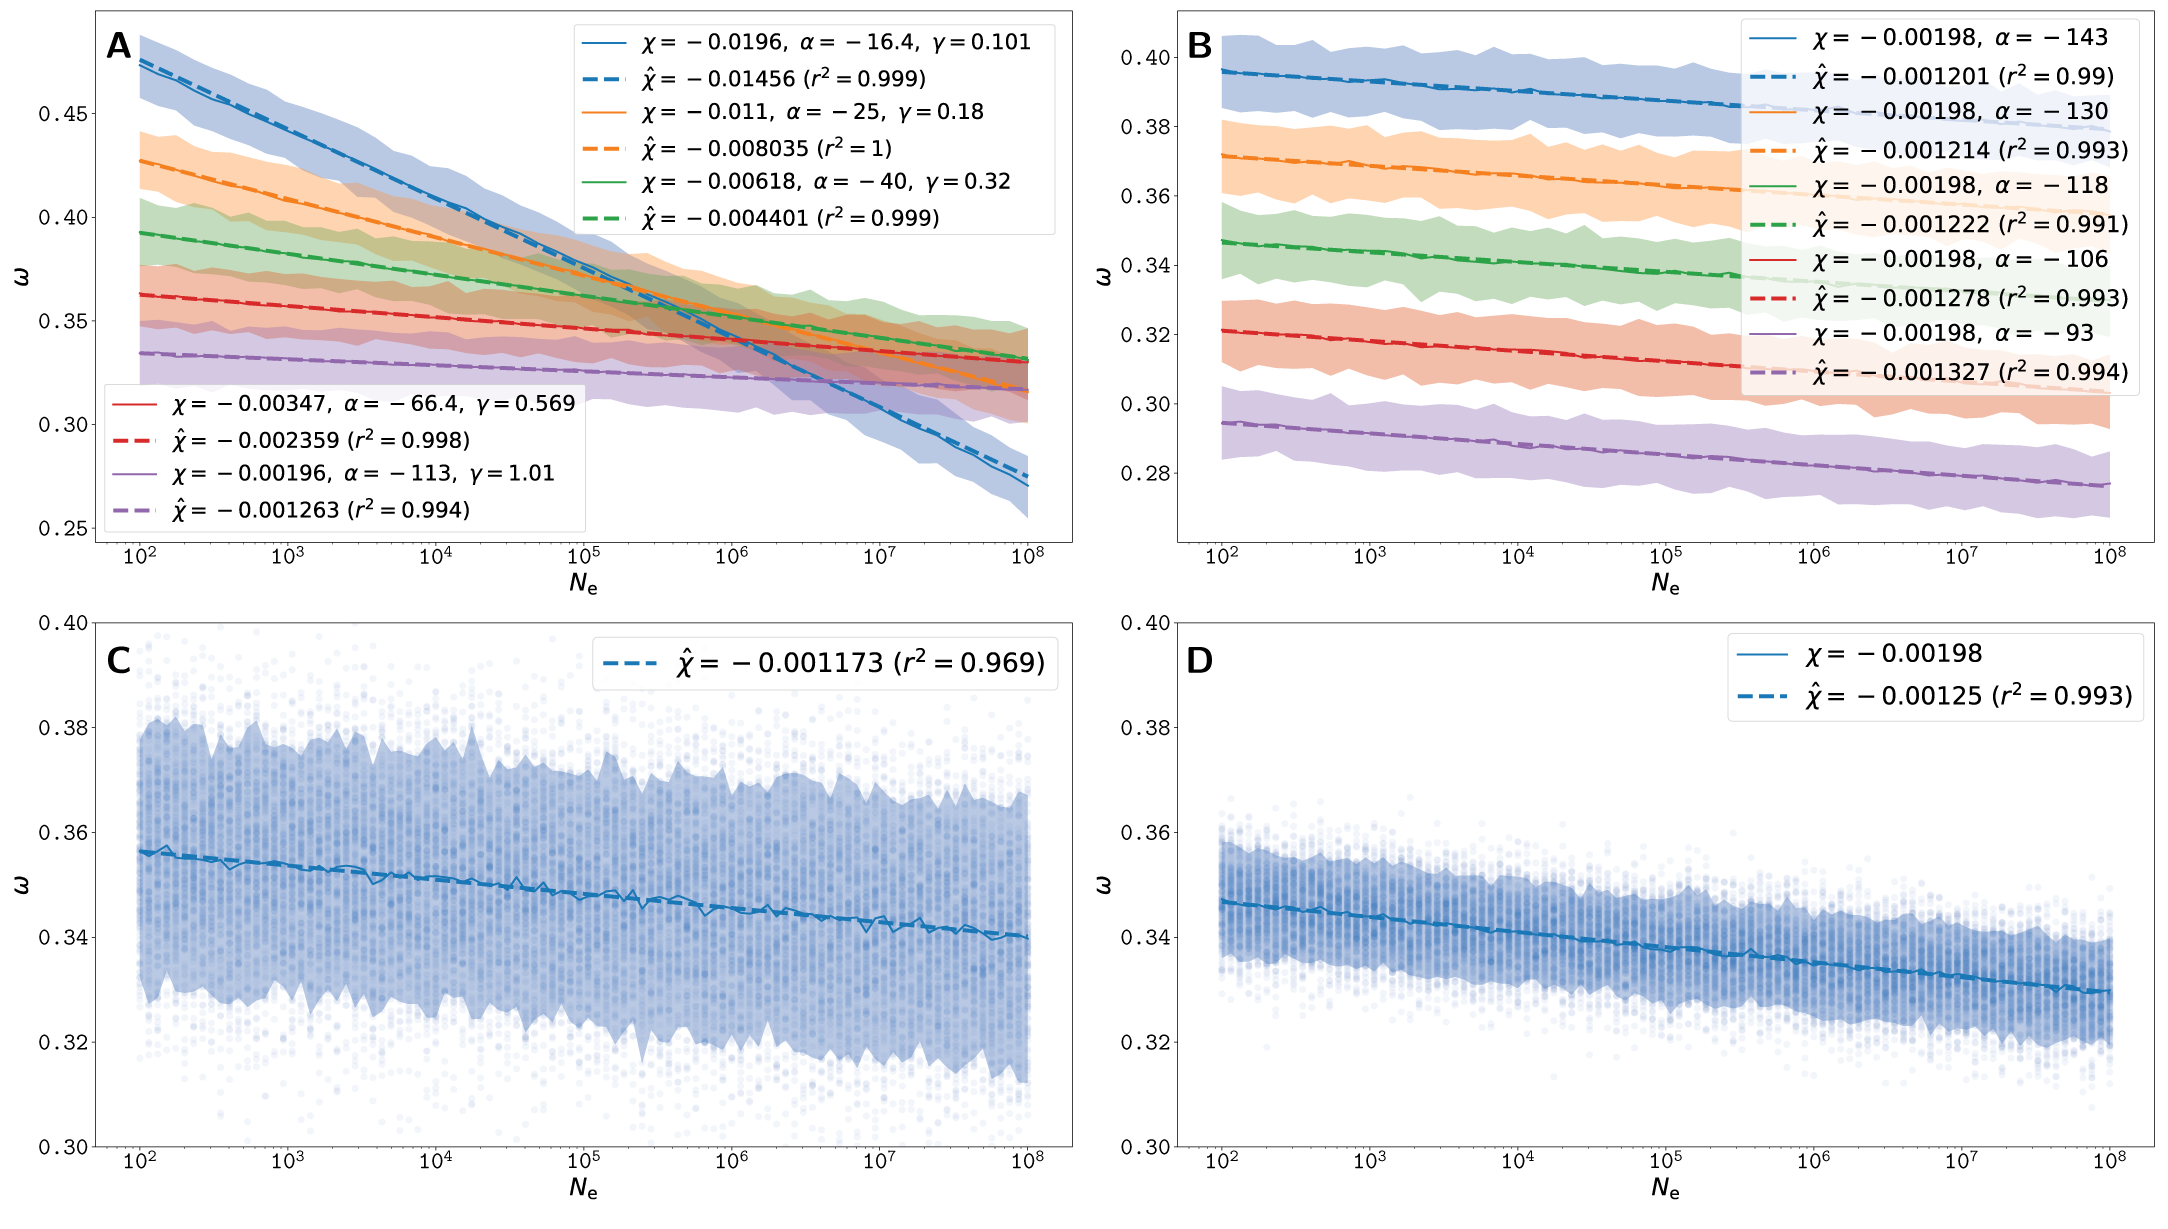
\includegraphics[width=0.9\textwidth] {artworks/Elasticity.png}
 \caption{
  \textbf{$\bm{\dnds}$ elasticity to change in $\bm{\Ne}$}.
  For each population size, $100$ simulations were performed and the average (solid line) and $90\%$ confidence interval (shaded area) are shown.
  Panel A. The fixed parameters are $\gamma=1$, $\Nsite=300$, $\beta=1.686$, and for each non-optimal amino-acid, $\gamma$ is scaled by the Grantham distance to the optimal amino-acid. $\alpha$ are given in the legend. Decreasing $\alpha$ (to more negative values) increases $\dnds$ but changes hardly the slope of the linear regression, as expected theoretically.
  $\dnds$ at equilibrium as a function of $\bm{\Ne}$ (log scale).
  Panel B. The fixed parameters are $\Nsite=300$ and $\beta=1.686$. Parameters $\alpha$ and $\gamma$ are given in the legend.
  $\gamma$ is increased and $\alpha$ is changed accordingly such that the equilibrium value $\x\eq$ is kept constant, by solving numerically equation \ref{eq:equilibrium}.
  The slope of $\dnds$-$\Ne$ relationship decreases proportionally to the inverse of $\gamma$, as predicted by our theoretical model.
  Panel C. In the model of 3D free energy of folding, $\dnds$ at equilibrium is weakly dependent on log-$\Ne$ but is not independent as claimed originally \cite{Goldstein2013}.
  This weak dependence matches the theoretical prediction of our additive free energy model that the linear relation (dashed line) has a slope equal to $(\beta \Nsite \gamma)^{-1} = 0.00198 \simeq 0.00124$.
  Bottom D, the fixed parameters are $\alpha=-118$, $\gamma=1$, $\Nsite=300$, $\beta=1.686$, and for each non-optimal amino-acid, $\gamma$ is scaled by the Grantham distance to the optimal amino-acid.
  Moreover, with the Grantham model, the $\dnds$ matches the empirical 3D model of Golstein \& Pollock and the theoretical prediction.
  \label{fig:GoldsteinVsToy}
 }
\end{mdframed}
\end{figure*}
\subsection*{Epistasis and time to relaxation}
Although the equilibrium value of $\dnds$ after changes in $\Ne$ is an important feature of the $\dnds$-$\Ne$ relationship, another parameter that is scarcely studied is the relaxation time to reach the new equilibrium $\dnds$ \cite{Jones2016}.
We observed in our simulations that the determining factor of the relaxation time is the number of sites $\Nsite$ (See Figure \ref{fig:relaxStability}).
Such observations match the theoretical prediction that high epistasis leads to faster return to equilibrium, since more opportunities are available.
In the case of a fitness landscape with epistasis, after a change in $\Ne$, any site that is used to climb either up or down the fitness landscape will have diminishing return in other sites of the sequences.
Not taking into account epistasis have the consequence of overestimating the relaxation time to return to equilibrium of $\dnds$ after changes in $\Ne$ .
Using a site-specific fitness landscape, where each amino-acid have different fitness, thus with no epistasis, the relaxation time is long since every site has to adapt to the new change in $\Ne$.
However, using a fixed distribution of fitness effect (DFE) does not suffer from underestimating the relaxation rate, since the effect is instantaneous (see Figure \ref{fig:relaxStability}).
\begin{figure*}[htb!]
\begin{mdframed}
 \centering
 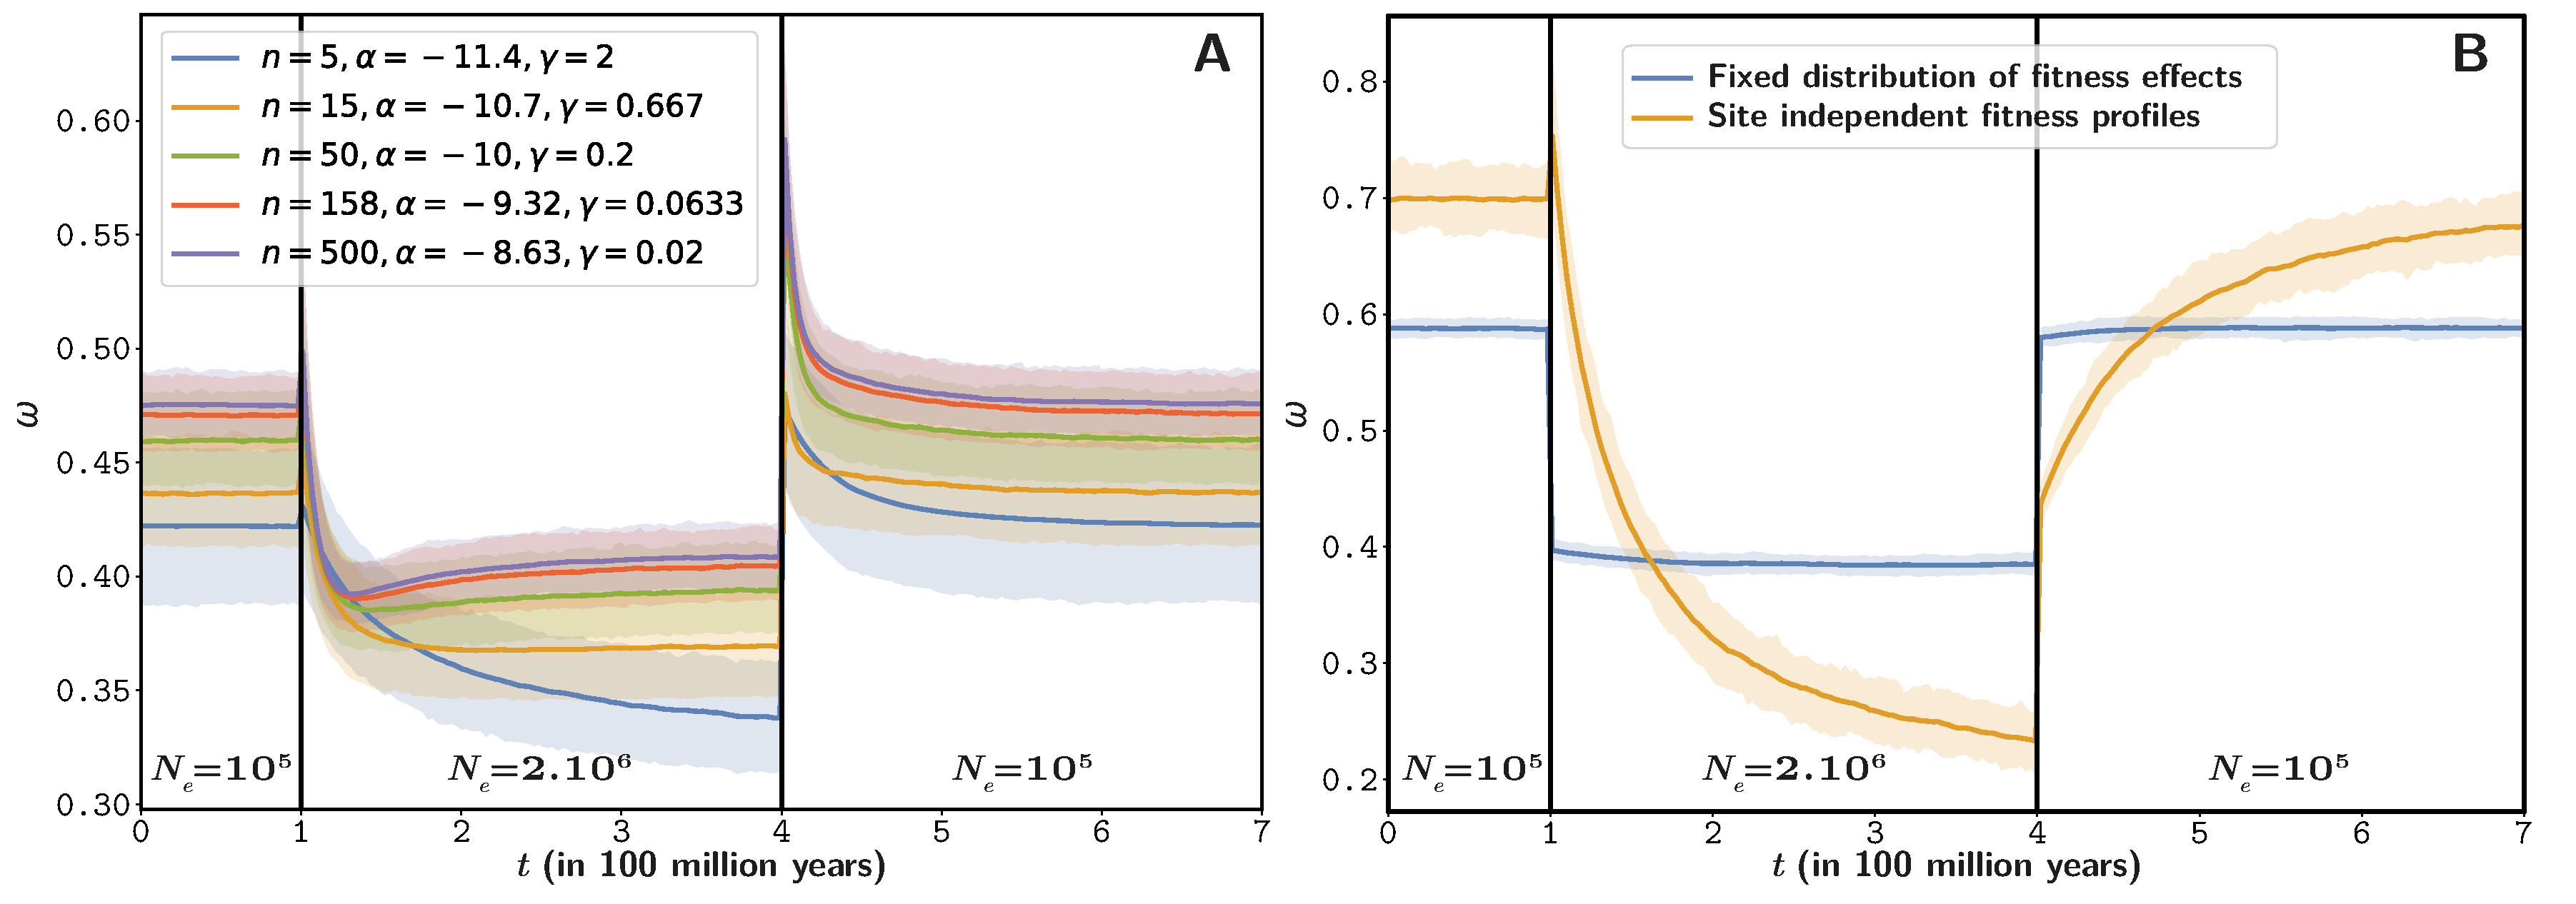
\includegraphics[width=0.9\textwidth] {artworks/Relaxation.pdf}
 \caption{
  \textbf{$\bm{\dnds}$ relaxation time to changes in $\bm{\Ne}$}.
  $\dnds$ relaxation after a brutal change in $\Ne$.
  Solid line corresponds to the average over replicates and the shaded area correspond to the $90\%$ interval among replicates. 
  The mutation rate ($\mu$) is $1e{-8}$ per year per site, and the total time of the computation is $700$ million years.
  Panel A. $\beta=1.686$, $\gamma=-10$ for all simulations. The number of sites is changed from $\Nsite=15$ to $\Nsite=158$, and the number of replicates ($r$) is changed accordingly such that the total number of sites ($\Nsite*r$) is kept constant.
  Moreover, $\gamma$ is changed according to $\Nsite$ such that the product $\gamma\Nsite$ is kept constant, thus the elasticity of the $\dnds$ to changes in $\Ne$ is kept constant.
  Finally, $\alpha$ is changed according to $\Nsite$ and $\gamma$ such that the equilibrium value $\x\eq$ is kept constant, by solving numerically equation \ref{eq:equilibrium}.
  Increasing $\Nsite$ implies a reduced time to reach the new equilibrium.
  Panel B. In context of a fixed fitness landscape, where each amino-acid has different fitness (site-specific profile), the time taken to reach the new equilibrium value of $\dnds$ after a change in $\Ne$ is long, such that relaxation rate is on the order of the mutation rate. In the context of a distribution of fitness effects, the relaxation time is non-existent.
 }
 \label{fig:relaxStability}
\end{mdframed}
\end{figure*}

Previous studies have argued that model of protein evolution should consider epistasis for various empirical reasons such as rate heterogeneity along the sequence, rate and time dependence of convergence, role of compensatory substitutions, prediction of deleterious mutations \cite{Goldstein2017}.
We argue that epistasis also have an important role the elasticity of $\dnds$ to changes in $\Ne$.
If epistasis is not taken into account, the elasticity of $\dnds$ is spread along time incompatible with biological evolution. \\
% Epistasis influence relaxation time


\section*{Discussion}
The negative relationship between the relative substitution rate of selected mutations ($\dnds$) and $\Ne$ has been predicted theoretically under the quasi-neutral theory of evolution.
Empirical data showed mitigated confirmation of this prediction, encouraging alternative explanatory mechanism.
One such explanation, developed in the context of genotype-phenotype-fitness map, demonstrated the absence of $\dnds$ elasticity to changes in $\Ne$ if the probabilities of phenotype changes are invariant to the current phenotype.
We argue that this assumption can be relaxed, and provide theoretical tools to derive the relationship between $\Ne$ and $\dnds$ in this context.
We apply our framework in the special case of fitness proportional to the proportion of folded proteins. \\
% Goal and theoretical results

Our theoretical results demonstrate that the relationship between $\dnds$ and $\Ne$ (in log space) is linear with a negative slope.
This slope is a function of molecular parameters of the model, and is inversely proportional to the product of the sequence size and the average change in conformational energy of destabilizing mutations. 
Based on empirical estimate of the molecular parameters, the elasticity of $\dnds$ to changes in $\Ne$ would be $\chi \simeq 0.002$.
Our compact theoretical results are supported by more complex simulations of protein evolution relaxing several assumptions.
% Our theoretical results are robsut to approximations

Particularly, our theoretical prediction match a numerical model of protein evolution, in which the free energy of the folded are unfolded conformations are computed using $3$D structures of the protein conformations.
Previous studies using this model presented an apparent lack of $\dnds$ elasticity to changes in $\Ne$ \cite{Goldstein2013}.
We argue the apparent lack of elasticity is in fact due to the subtle relation, and require extensive computation to be detected.\\
% Goldstein \& Pollock model don't have a null elasticity

Empirically, inference of the $\dnds$ elasticity in Primates, using polymorphism and divergence data estimated $\chi \simeq $, approximately $X$ times greater than our theoretical prediction \cite{Brevet2019}.
More empirical data across clades would be required to infirm such model, but in the light of empirical data estimating the relationship between $\Ne$ and $\dnds$, models based on the probability of folding are not reasonably fitted.\\
% Our result show the fitness proportional to proportion of folded folding is at odd with empirical data

Furthermore, our theoretical results manifest that the relationship between $\Ne$ and $\dnds$ is the same as the relationship between protein abundance and $\Ne$, whenever protein fitness is determined by the deleterious effect of unfolded proteins.
As such, dataset relating $\dnds$ to $\Ne$ and protein can be used confirm or infirm this model.\\
% Stress the importance that elasticity is valid for Ne and protein abondance

Notably, theoretical approximations apply more broadly to protein-protein interactions (See Supplementary Materials), where protein may either be in free form or engaged in a non-specific interaction. 
In non-specific interactions, stable site are hydrophilic amino-acid and unstable site are hydrophobic amino-acid at the protein surface.
Fitting this model with empirical estimates \cite{Zhang2008}, we obtain an elasticity of $\chi = 0.2$ (See Supplementary Materials) thus a much stronger response than under the model based on conformational stability. 
This effect is due to less sites in the protein being involved in protein-protein interaction than for conformational stability, in addition to the lower energy engaged in the contacts.
As such, in light of empirical data available, the assumption that protein fitness is determined such as to avoid non-specific interaction is more likely than the assumption that protein fitness is determined by the deleterious effect of unfolded proteins. \\
% Protein-protein interactions

% DFE can also be used to fit to empirical data - Shall we present this ?

\section*{Materials \& Methods}
Protein sequence evolution is simulated under an origin-fixation model \cite{McCandlish2014}, where one sequence represent the whole population.
From the resident DNA sequence $\ci$, we define $\setNeighbors$ as the set of all possible mutant that are one nucleotide away from $\ci$, and were mutant sequences containing a stop codon are excluded.
For a protein of $\Nsite$ amino-acid sites, $\left| \setNeighbors \right| \leq 9 \Nsite$, since each codon has a maximum of $9$ possible mutant codons that are one mutation away and that are not stop codon.
For each mutant sequence $\cj \in \setNeighbors$, we compute its fitness and subsequently the selection coefficient of the mutant:
\begin{equation}
s \left( \ci,\cj\right) = \dfrac{ f \left(\cj \right) - f \left(\ci\right) }{f\left( \ci \right)}.
\end{equation}
The next event of mutant invading the population, and the time to reach such event is chosen using Gillespie algorithm, according to the rates of substitution between sequences:
\begin{equation}
\submatrix_{\itoj} = \mu_{\itoj} \dfrac{4 \Ne s \left( \ci,\cj\right)}{1 - \e^{-4 \Ne s \left( \ci,\cj\right)}}, 
\end{equation}
where $\mu_{\itoj}$ is the mutation rate between $\ci$ and $\cj$, determined by the underlying $4x4$ nucleotide mutation rate matrix, and ${\submatrix_{\itoj}} = \mu_{\itoj}$ in the case of synonymous substitutions.
Various optimization are implemented to reduce the computation time of mutant's fitnesses.
The simulation starts with a burn-in period to reach mutation-selection-drift equilibrium.
\subsection*{Models of fitness function}
\label{MatMet:folding}
Under a simulation of protein folding with an additive model of free energy, the protein's difference in free energy between folded and unfolded state is given by:
\begin{equation*}
\deltaG\left(\ci\right) = \alpha + \Nsite \gamma * \x\left(\ci\right), 
\end{equation*}
where $0 \leq \x\left(\ci\right) \leq 1$ is the distance of $\ci$ to the optimal sequence.
For each site of sequence, the optimal amino-acids are chosen randomly at initialization, and the distance between the current amino-acid and the optimal is scaled by the Grantham amino-acid distance \cite{Grantham1974}.
Wrightian fitness is defined as the probability of our protein to be in the folded state, given by the Fermi-Dirac distribution: 
\begin{equation}
f(\deltaG\left(\ci\right)) = \dfrac{e^{-\beta \deltaG\left(\ci\right) }}{1 + e^{-\beta \deltaG\left(\ci\right) }} = \dfrac{1}{1 + e^{\beta \deltaG\left(\ci\right) }}, 
\end{equation}
where $\beta$ is the inverse of the temperature ($\beta=1/kT$).\\

Under a simulation with site independent fitness profiles, a fitness profile give a fitness for each amino-acid (vector of size $20$).
Each site of the protein has a specific amino-acid fitness profile.
Overall, the protein phenotype is computed as the sum of site-specific selection coefficient, obtained by accessing the amino-acid present at each site of the protein.
The selection coefficient of the mutant $\cj$ is:
\begin{equation}
s \left( \ci,\cj\right) = \sum_{1 \leq \site \leq \Nsite} \ln \left( \dfrac{G_{\site} \left(\cj(\site) \right)}{G_{\site} \left(\ci(\site) \right)} \right) ,
\end{equation}
where $G_{\site}$ is the fitness profile at site $\site$, obtained in empirical experiment \cite{Bloom2017}.


Under simulation with a fixed distribution of fitness effects (DFE), the selection coefficient of the mutant $\cj$ is gamma distributed (shape $\beta > 0$):
\begin{equation}
- s \left( \ci,\cj\right) \sim \text{Gamma} \left( \bar{|s|}, \beta \right)
\end{equation}
\subsection*{$\bm{\dnds}$ along the simulation}
From the set of mutants $\setNeighbors$ that is one nucleotide away from $\ci$, we define the subsets $\setNonSynNeighbors$ and $\setSynNeighbors$ that are respectively the set of non-synonymous and synonymous mutants, where $\setNonSynNeighbors \cup \setSynNeighbors = \setNeighbors$.
As in previous works \cite{Spielman2015a, DosReis2015, Jones2016}, the ratio of non-synonymous over synonymous substitution rates of the sequence is defined as :
\begin{align}
\dnds(t) &= \dfrac{\sum_{\cj \in \setNonSynNeighbors} \submatrix_{\itoj}}{\sum_{\cj \in \setNonSynNeighbors} \mu_{\itoj}} \left( \dfrac{\sum_{\cj \in \setSynNeighbors} \submatrix_{\itoj}}{\sum_{\cj \in \setSynNeighbors} \mu_{\itoj}} \right)^{-1}\\
 &= \dfrac{\sum_{\cj \in \setNonSynNeighbors} \mu_{\itoj} \dfrac{4 \Ne s \left( \ci,\cj\right)}{{1 - \e^{-4 \Ne \left( \ci,\cj\right)} }}}{\sum_{\cj \in \setNonSynNeighbors} \mu_{\itoj}} 
\end{align}
And $\dnds$ is taken as the average of the time-dependent $\dnds(t)$ along the simulation.
\subsection*{Reproducibility}
The simulators written in C++ are publicly available under MIT license at \url{https://github.com/ThibaultLatrille/SimuEvol}.
The scripts and instructions necessary to reproduce the experiments are available at \url{https://github.com/ThibaultLatrille/GenotypePhenotypeFitness}.
\bibliographystyle{apalike}
\bibliography{refs-codons,refs-cds}

\end{document}